\documentclass[letterpaper, 10 pt, conference]{ieeeconf}
\IEEEoverridecommandlockouts
\overrideIEEEmargins   

\newcommand\independent{\protect\mathpalette{\protect\independenT}{\perp}}
\def\independenT#1#2{\mathrel{\rlap{$#1#2$}\mkern2mu{#1#2}}}


\usepackage{cite}
\usepackage{amsmath,amssymb,amsfonts}
\usepackage{algorithm}
\usepackage{algpseudocode}
\usepackage{graphicx}
\usepackage{textcomp}
\usepackage{xcolor}
\usepackage{tabularx}
\newtheorem{Theorem}{Theorem}
\newtheorem{Lemma}{Lemma}
\newtheorem{Assumption}{Assumption}
\newtheorem{Definition}{Definition}
\newtheorem{Corollary}{Corollary}
\newtheorem{Remark}{Remark}
\usepackage{graphicx}
\usepackage{array}
\usepackage{caption}
\usepackage{subcaption}
\usepackage{adjustbox}
\usepackage[utf8]{inputenc}
\usepackage{mathtools}
\usepackage{balance}
\usepackage{hyperref}
\usepackage{authblk}


\def\Ac{{\mathcal A}}
\def\Abb{{\mathbb A}}
\def\Abf{{\mathbf A}}
\def\abf{{\mathbf a}}

\def\Bc{{\mathcal B}}
\def\Bbb{{\mathbb B}}
\def\Bbf{{\mathbf B}}
\def\bbf{{\mathbf b}}

\def\Cc{{\mathcal C}}
\def\Cbb{{\mathbb C}}
\def\Cbf{{\mathbf C}}
\def\cbf{{\mathbf c}}

\def\Dc{{\mathcal D}}
\def\Dbb{{\mathbb D}}
\def\Dbf{{\mathbf D}}
\def\dbf{{\mathbf d}}

\def\Ec{{\mathcal E}}
\def\Ebb{{\mathbb E}}
\def\Ebf{{\mathbf E}}
\def\ebf{{\bf e}}

\def\Fc{{\mathcal F}}
\def\Fbb{{\mathbb F}}
\def\Fbf{{\mathbf F}}

\def\Gc{{\mathcal G}}
\def\Gbb{{\mathbb G}}
\def\Gbf{{\mathbf G}}
\def\gbf{{\mathbf g}}


\def\Hc{{\mathcal H}}
\def\Hbb{{\mathbb H}}
\def\Hbf{{\mathbf H}}
\def\hbf{{\mathbf h}}

\def\Ic{{\mathcal I}}
\def\Ibb{{\mathbb I}}
\def\Ibf{{\mathbf I}}

\def\ei{{  {\mathbf e}_{\Psi} }}

\def\Jc{{\mathcal J}}
\def\Jbf{{\mathbf J}}
\def\Jbb{{\mathbb J}}

\def\Kc{{\mathcal K}}

\def\Lc{{\mathcal L}}
\def\Lbb{{\mathbb L}}
\def\Lrm{{\rm L}}
\def\Lbf{{\mathbf L}}
\def\Lfr{{\mathfrak L}}

\def\Mc{{\mathcal M}}
\def\Mbb{{\mathbb M}}
\def\Mbf{{\mathbf M}}
\def\mbf{{\mathbf m}}

\def\Nc{{\mathcal N}}
\def\Nbb{{\mathbb N}}
\def\Nbf{{\mathbf N}}

\def\Oc{{\mathcal O}}
\def\Obb{{\mathbb O}}
\def\Obf{{\mathbf O}}

\def\Pc{{\mathcal P}}
\def\Pbb{{\mathbb P}}
\def\Pbf{{\mathbf P}}
\def\pbf{{\mathbf p}}

\def\Qc{{\mathcal Q}}
\def\Qbb{{\mathbb Q}}
\def\Qbf{{\mathbf Q}}


\def\Rc{{\mathcal R}}
\def\Rbb{{\mathbb R}}
\def\Rbf{{\mathbf R}}
\def\Rfr{{\mathfrak R}}

\def\Sc{{\mathcal S}}
\def\Sbf{{\mathbf S}}
\def\sbf{{\mathbf s}}
\def\Sbb{{\mathbb S}}

\def\Tc{{\mathcal T}}
\def\Tbb{{\mathbb T}}
\def\Tbf{{\mathbf T}}
\def\tbf{{\mathbf t}}

\def\Uc{{\mathcal U}}
\def\Ubb{{\mathbb U}}
\def\Ubf{{\mathbf U}}
\def\ubf{{\mathbf u}}

\def\Vc{{\mathcal V}}
\def\Vbb{{\mathbb V}}
\def\Vbf{{\mathbf V}}
\def\vbf{{\mathbf v}}

\def\Wc{{\mathcal W}}
\def\Wbb{{\mathbb W}}
\def\Wbf{{\mathbf W}}
\def\wbf{{\mathbf w}}

\def\Xc{{\mathcal X}}
\def\Xbb{{\mathbb X}}
\def\Xbf{{\mathbf X}}
\def\xbf{{\mathbf x}}

\def\Yc{{\mathcal Y}}
\def\Ybb{{\mathbb Y}}
\def\Ybf{{\mathbf Y}}
\def\ybf{{\mathbf y}}

\def\Zc{{\mathcal Z}}
\def\Zbb{{\mathbb Z}}
\def\Zbf{{\mathbf Z}}
\def\zbf{{\mathbf z}}

\def\mat{{\mathbb M}}
\def\nat{{\mathbb N}}

\def\Xibf{{\bf \Xi}}


\def\Th{{\Theta}}
\def\th{{\theta}}
\def\ze{{\zeta}}
\def\Ze{{\zeta}}
\def\ga{{\gamma}}
\def\Ga{{\Gamma}}

\def\pa{{\partial}}

\def\ep{{\epsilon}}

\def\om{{\omega}}
\def\Om{{\Omega}}

\def\Lmb{{\Lambda}}


\def\half{{\frac{1}{2}}}

\def\lam{{\lambda}}
\def\Lam{{\Lambda}}
\def\stm{{\setminus}}

\def\Sg{{\Sigma}}
\def\0{{\bf 0}}
\def\ker{{\rm ker}\,}
\def\dim{{\rm dim}\,}
\def\defe{\stackrel{\triangle}{=}}



\newcommand{\st}{\stackrel{J}{\approx}}
\newcommand{\stt}{\stackrel{I}{\approx}}
\newcommand{\bitem}{\begin{itemize}}
\newcommand{\eitem}{\end{itemize}}
\newcommand{\btabular}{\begin{tabular}}
\newcommand{\etabular}{\end{tabular}}
\newcommand{\bcenter}{\begin{center}}
\newcommand{\ecenter}{\end{center}}
%\newcommand{\be}{\begin{equation}}
%\newcommand{\ee}{\end{equation}}
\newcommand{\bea}{\begin{eqnarray}}
\newcommand{\eea}{\end{eqnarray}}
\newcommand{\bean}{\begin{eqnarray*}}
\newcommand{\eean}{\end{eqnarray*}}

\newcommand{\ba}{\left. \begin{array}}
\newcommand{\ea}{\\ \end{array} \right.}
\newcommand{\bab}{\left[ \begin{array}}
\newcommand{\eab}{\\ \end{array} \right]}
\newcommand{\bap}{\left( \begin{array}}
\newcommand{\eap}{\\ \end{array} \right)}
\newcommand{\bbm}{ \begin{bmatrix}}
\newcommand{\ebm}{\\ \end{bmatrix} }
\newcommand{\bear}{\begin{array}}
\newcommand{\eear}{\\ \end{array}}


\newcommand{\tcr}{\textcolor{red}}
\newcommand{\tcb}{\textcolor{black}}
\newcommand{\ovl}{\overline}
\newcommand{\ul}{\underline}
\newcommand{\wt}{\widetilde}
\newcommand{\td}{\tilde}
\newcommand{\bs}{\boldsymbol}

%\newcommand{\br}{\breve}

\newcommand{\noi}{\noindent}
\newcommand{\non}{\nonumber}
\newcommand{\bb}{\cite}
\newcommand{\Lra}{\Leftrightarrow}
\newcommand{\Ra}{\Rightarrow}
\newcommand{\La}{\Leftarrow}
\newcommand{\lra}{\leftrightarrow}
\newcommand{\ra}{\rightarrow}
\newcommand{\la}{\leftarrow}
\newcommand{\ran}{\rangle}
\newcommand{\lan}{\langle}
\newcommand{\Lolra}{\Longleftrightarrow}
\newcommand{\Lora}{\Longrightarrow}
\newcommand{\Lola}{\Longleftarrow}
\newcommand{\lolra}{\longleftrightarrow}
\newcommand{\lora}{\longrightarrow}
\newcommand{\lola}{\longleftarrow}
\newcommand{\btd}{\bigtriangledown}
\newcommand{\btu}{\bigtriangleup}
%\renewcommand{\theequation}{\arabic{section}.\arabic{equation}}
\newcommand{\ad}{{\rm \;\;\;\; and \;\;\;\;\;}}
\newcommand{\Qcd}{\hfill{\Qced}}
\newcommand{\hbb}{\hfill{\box}}
\def\Qced{{\ \vrule width 1.5mm height 1.5mm \smallskip}}

\font\myownfont=cmr17 scaled \magstep5
\def\psfancypar#1#2{\def\biginitial#1{{\myownfont#1}}%
  \def\makeinitial#1{\setbox8\hbox{\strut\vbox to 1.3ex
    {\hbox{\biginitial#1}\vskip -4pc plus 3.5pc minus 3.5pc}}}%
  \makeinitial#1%
  \ifdim\parindent>1.3\wd8\dimen8=\parindent
     \else\dimen8=1.3\wd8\fi
  \hangindent=\dimen8\hangafter=-2
  \noindent
  \strut\hskip-1\dimen8\box8{\sc#2}}%

\def\scalefig#1{\epsfxsize #1\textwidth}
\def\scalefigy#1{\epsfysize #1\textwidth \epsfxsize 0.7\textwidth}

\newcounter{subequation}
\def\beasub{\addtocounter{equation}{+1}
\setcounter{subequation}{\value{equation}}
\setcounter{equation}{0}
\renewcommand{\theequation}{\arabic{subequation}\alph{equation}}
\begin{eqnarray}}
\def\eeasub{\end{eqnarray}
\setcounter{equation}{\value{subequation}}
\renewcommand{\theequation}{\arabic{equation}}}

%\newcommand{\over}{\overline}
\newcommand{\under}{\underline}
\newcommand{\mb}{\mathbf}
\newcommand{\mrg}{\mathring}
\newcommand{\tb}{\textbf}



% \setlength{\abovedisplayskip}{1pt}
% \setlength{\belowdisplayskip}{1pt}
\DeclareMathOperator*{\argmax}{arg\,max}

\newtheorem{theorem}{Theorem}[section]
\newtheorem{lemma}[theorem]{Lemma}
\newtheorem{problem}[theorem]{Problem}
\newtheorem{proposition}[theorem]{Proposition}
\newtheorem{corollary}[theorem]{Corollary}
\newtheorem{definition}[theorem]{Definition}
\newtheorem{remark}[theorem]{Remark}
\newtheorem{assumption}[theorem]{Assumption}


\DeclareMathOperator*{\argmin}{arg\,min}
\DeclareMathOperator*{\logdet}{log\,det}

\makeatletter
\newcommand{\linebreakand}{%
\end{@IEEEauthorhalign}
\hfill\mbox{}\par
\mbox{}\hfill\begin{@IEEEauthorhalign}
}
\makeatother

%\title{\LARGE \bf Mapping spatio-temporal fields with informative path planning by multiple mobile robots }
\title{\LARGE \bf Data-driven model of port-Hamiltonian Systems with algebraic constraints}

\author{Binh Nguyen$^{1}$, Truong X. Nghiem$^{1}$
\author[1]{Binh Nguyen}
\author[2]{Truong Nghiem}
% \affil[1]{Department of Engineering, Texas A\&M University–Corpus Christi, Corpus Christi, TX 78412, USA}
% \affil[2]{Institute of Innovation, Science and Sustainability, Federation University Australia, Churchill, VIC 3842, Australia}
% \affil[3]{School of Informatics, Computing, and Cyber Systems, Northern Arizona University, Flagstaff, AZ 86011, USA}
\thanks{$^1$The  Department of Electrical and Computer Engineering, College of Engineering and Computer Science, University of Central Florida, Orlando, FL 32816, USA}
}
\date{September 2024}



\begin{document}

\maketitle


\begin{abstract}
\end{abstract}

\section{Introduction}

Basic Introduction Port-Hamiltonian Systems (PHS) has been given in \cite{schaftPortHamiltonianSystemsTheory2014}. Survey papers on learning control techniques including reinforcement learning (RL), iterative control and for PHSs 
\cite{nageshraoPortHamiltonianSystemsAdaptive2016,rashadTwentyYearsDistributed2020,cherifiOverviewRecentMachine2020}. 

Reduced-order PHs \cite{wuReducedOrderLQG2021,schwerdtnerOptimizationbasedModelOrder2023}


Gassian Process approach for modelling PHSs
\cite{beckersGaussianProcessPortHamiltonian2022,beckersLearningSwitchingPortHamiltonian2023} and then Bayesian Control for PHSs \cite{beckersDataDrivenBayesianControl2023a}.
%%

The first attemp using neural network to describe Hamiltonian systems
\cite{greydanusHamiltonianNeuralNetworks2019a}. 
%%
Following the concept,
\cite{nearyCompositionalLearningDynamical2023,eidnesPseudoHamiltonianNeuralNetworks2023,desaiPortHamiltonianNeuralNetworks2021,duongPortHamiltonianNeuralODE2024} have applied physics-informed neural network (PINN) with well-chosen learning biases for modelling PHSs has established foundation of port-Hamiltonian neural network (PHNN).

Data-driven identificaiton of PHSs 
\cite{rettbergDatadrivenIdentificationLatent2024,otterdijkLearningSubsystemDynamics2024}

\subsection{Related Works}

\noindent\cite{otterdijkLearningSubsystemDynamics2024} {\bf Pros:} can work to input-output data, interconnection of port-Hamiltonian systems (composite learning or identificaiton). {\bf Cons:} No uncertatinty quantification. {\bf Framework:} PHNN + composite PHSs

\noindent\cite{nearyCompositionalLearningDynamical2023} {\bf Pros:} can work to interconnection of port-Hamiltonian systems. {\bf Cons:} Use state variables and no uncertatinty quantification. {\bf Framework:} {\bf Framework:} PHNN + composite PHSs

\noindent\cite{beckersGaussianProcessPortHamiltonian2022} {\bf Pros:} uncertatinty quantification with noised data. {\bf Cons:} Use state variables, prior GP assumption. {\bf Framework:} {\bf Framework:} GP-PHSs

\noindent\cite{altawaitanHamiltonianDynamicsLearning2024} focuses only on nonhomolomic systems, no constraint-preservation is given

\noindent\cite{vanderschaftGeneralizedPortHamiltonianDAE2018,
vanderschaftDiracLagrangeAlgebraic2020} Lagrangian constraints and Dirac constraints.

All above works do not consider constrained port-Hamiltonian systems.

\subsection{Contribution}

\section{Constrained pHs}
\subsection{Problem statement}
\begin{figure}
    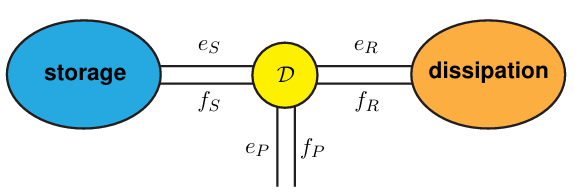
\includegraphics[width = \linewidth]{pH.PNG}
    \caption{Structure of Port-Hamiltonian system}
\end{figure}


\begin{definition}[Constant Dirac Structure \cite{schaftPortHamiltonianSystemsTheory2014}] 
    A Dirac structure is
    a subspace $\Dc \subset \Sc \times \Sc^\star$ such that $\Dc = \Dc^{\independent}$, where $^{\independent}$ denotes
    the orthogonal companion with respect to the bilinear form $\langle\cdot,\cdot\rangle_+$
\end{definition}

\begin{definition}[Generalized pH DAE System \cite{vanderschaftGeneralizedPortHamiltonianDAE2018}] Consider a Dirac
    structure $\Dc \subset \Sc \times \Sc^\star$ and a Lagrangian subspace $\Lc \subset \Sc \times \Sc^\star$.
    This defines the generalized port-Hamiltonian DAE system (briefly,
    gpH DAE system) $(\Dc, \Lc)$, with dynamics given by    
    \begin{align}
        (\dot x, e) \in \Dc, (x,e) \in \Lc
    \end{align}
\end{definition}

By letting
$e_S = \frac{\pa H}{\pa \xbf}$, $f_S = -\dot\xbf$,
Consider input-state model of pHs as follows
\begin{align}
    \dot \xbf = (J - R)\frac{\pa H}{\pa \xbf} + G \ubf + 
    \bbm 0 \\ A \bs\lambda \ebm \label{org_str}   
    \\
    A^\top \frac{\pa H}{\pa \xbf} = 0.
    \label{org_cstr}
\end{align}
Where $\xbf \in \Rbb^n$, $J = J^\top$ is a skew matrix, $R = R^\top$ stands for positive.
%%
As a special case of input-output algebraic constraints  \cite[Chapter 8]{schaftPortHamiltonianSystemsTheory2014}.

From \eqref{constraints}, $\frac{\pa H}{\pa \xbf}$ must be lie in the raw space of $A$, let us define a constraint set $\Xc$ as a set of all $\xbf$ satisfied \eqref{constraints}.
%%
Let us select $c$ basic vectors $\sbf_i$ of $\Xc$, and define  matrix
$B = [s_1^\top;\dots;s_c^\top] \in \Rbb^{n\times c}$ which satisfies (\ref{BA}).
\begin{align}
    B A = 0.
    \label{BA}
\end{align}

{\bf Problem 1:} For given dataset $(\xbf, \ubf)$ and assume that $A(\xbf)$ is known, estimate $H(\xbf)$ and parameters $\phi_J, \phi_R, \phi_G$ coressponding to matrices $J,R,G$ such that the structure \eqref{org_str} and constraint \eqref{org_cstr} are presevered.


\subsection{Proposed approach}

Neural ODE with specific structures.

Define an approximation of Hamiltonian function
\begin{align}
    H(\xbf) = \sum_i^c NN_i(\xbf) \sbf_i^\top
\end{align}
Design $c$ neural network $NN_i(\xbf)$ such that
with $[NN_i(\xbf)]_j s_{ij} \geq 0$ where $\sbf_i = [s_{ij}]_{1\leq j\leq c}$.

\section{nonhomolomic Euler-Lagrangian Systems}
Let us consider a mechanical system with $n$ degrees of freedom, described by $n$ measurable configuration variables $\qbf = [q_1,q_2,\dots,q_n]^\top$. Accordingly, kinetic energy of the mechanical system is given by $K(\dot\qbf) = $
$\frac{1}{2} \dot\qbf^\top M(\qbf) \dot\qbf$ where $M(\qbf) = [M_{ij}(\qbf)] \in \Rbb^{n \times n}$ denotes the generalized mass matrix. In the light of \cite{}, we define the Lagrangian function $L(\qbf,\dot \qbf)$ in the following form
\begin{align}
    L(\qbf,\dot \qbf) = K(\dot\qbf) - U(\qbf)
\end{align}
where $U(\qbf)$ stands for potential energy of the mechanical system. This paper assume that there are nonhomolomic constraints of velocity $\dot \qbf$ as 
\begin{align}
    A^\top(\qbf) \dot\qbf = 0
\end{align}

Euler-Lagrange equations:
\begin{align}
    \frac{d}{dt}\left(\frac{\pa L}{\pa \dot\qbf}\right) - \frac{\pa L}{\pa \qbf} = A(\qbf) \bs\lambda + B(\qbf) \ubf
\end{align}
Defining the generalized momenta:
\begin{align}
    \pbf = \frac{\pa L}{\pa \dot \qbf} = M(\qbf)\dot \qbf
    \label{constraints}
\end{align}


Constrained Port-Hamiltonian is given by
\begin{align}
    \dot\qbf &= \frac{\pa H}{\pa \pbf},
    \\
    \dot\pbf & = -\frac{\pa H}{\pa \qbf} + A(\qbf) \bs\lambda + B(\qbf) \ubf,
    \\
    0 &= A^\top(\qbf) \frac{\pa H}{\pa\pbf}(\pbf,\qbf)
\end{align}
with $H(\qbf,\pbf) = \frac{1}{2} \pbf^\top M^{-1}(\qbf) \pbf + U(\qbf)$.

{\bf Assumption:} 

{\bf Problem 2:} From data $\{\qbf^\tau\}_{\tau\geq 0}$ and $\{\dot\qbf^\tau\}_{\tau\geq 0}$ up to time $t$ ($\tau \leq t$), 
learn parameters $\phi_M$ in matrix $M$ and provides predictions (for $\tau > t$) such that the nonhomolomic constraints \eqref{constraints} is satisfied.

\section{approach}

\bibliography{References}
\bibliographystyle{IEEEtran}

\end{document}